We briefly present the data on which this work is based on. The first instrument we've studied is the following European Call Option, written on an equity stock:

\begin{table}[H]
    \centering
    \begin{tabular}{|c|c|c|c|c|}
        \hline
        Strike & Underlying & Dividend & Volatility & TTM \\
        \hline
        1.05 & 1 & 2\% &21\% & 4 months \\
        \hline
    \end{tabular}
    \caption{European Call Option}
    \label{tab:market data}
\end{table}

We assume the zero rate in the market is $r = 2.5\%$. 
The holder of the option will take physical delivery of the underlying and is purchasing 1 Million contracts. 

\section{Question (a) Call Option Price}
We've applied three different methodologies to price the option described above:

\begin{itemize}
\item The \textsc{MATLAB} function \textit{blkprice}, which returns the option price according to the closed formula derived in \cite{black}.

\item the Cox-Ross-Rubenstein \textit{(CRR)} Tree Approach: the necessary parameters for pricing were defined, including the number of timesteps, up factor, down factor, and up/down probabilities. The option price was obtained by discounting the payoffs, starting from the terminal nodes and working backward through the tree, as described in the authors paper \cite{CRR}.

\item Monte Carlo Method: we generated 100 normal random variables in order to simulate the future possible paths of the underlying. We computed their corresponding prices under the risk neutral measure and their mean. We noticed that, with this limited sample of random variables, the price of the Call option was significantly different from the actual price (the one computed with the \textit{blkfunction}).
\end{itemize}

The price of the instrument using each one of the method is reported in the table below. The first row registers the price of one single contract, while the second one the price of 1 Millions of them.

\begin{table}[htpb]
    \centering
    \begin{tabular}{|| c | c | c ||}
    \hline
        \textbf{blkprice} & \textbf{CRR} & \textbf{MonteCarlo} \\
        0.02887443 & 0.02880214 & 0.04331091 \\
        28874.43 & 28802.14 & 43310.91 \\
    \hline
    \end{tabular}
    \caption{The results of the Monte Carlo simulation may vary depending on the seed used by the random number generator. We have chosen, for reproducibility, to set the seed in \textsc{MATLAB} to \textit{rng("default")}.}
    \label{tab:price_a}
\end{table}

\section{Question (b),(c) Errors of MC and CRR methods}
Our aim is to select $M$ (number of time steps in CRR and of normal random variables in Monte Carlo) in order to ensure that the error stayed below the spread $(1bp)$. We first plotted the error of the CRR Tree approach, considering the difference in absolute value with respect to the exact value. In this case we observed that it is decreasing as 1/M. Then we did the same for the error of the Monte Carlo simulation, computing it as the standard deviation of the Monte Carlo prices (since the standard deviation is an unbiased estimator of MC prices). In this situation the decrease behaves as $1/\sqrt{M}$.
Observing the graphs below:
\begin{itemize}
\item CRR approach: the desired M suggested by the figure is between 64 (\( 2^6 \)) and 128 (\( 2^7 \)); but, knowing that the error is not monotone decreasing, we noticed that selecting M equal to 18 the error was already less than 1 bp.

\item Monte Carlo simulation: the desired M suggested by the figure is between \( 10^5 \) and \( 10^6 \), hence a great choice would be $M=5\cdot  10^5$

\end{itemize}

\begin{figure}[htb!]
\centering
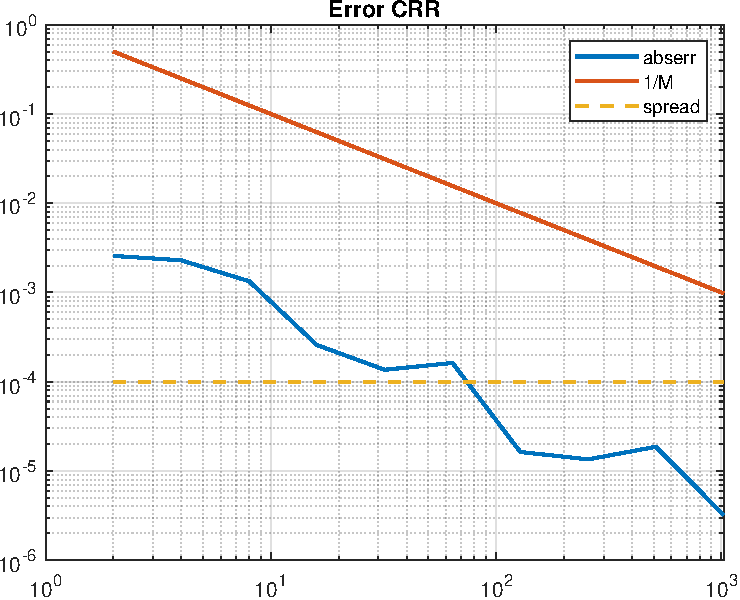
\includegraphics[width=0.45\linewidth]{imgs/err_crr.pdf}
\quad
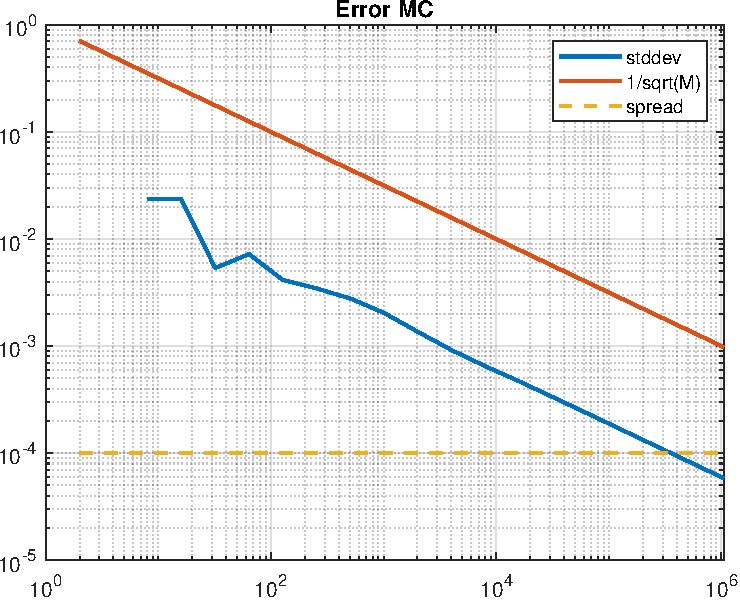
\includegraphics[width=0.45\linewidth]{imgs/err_mc.pdf}
\caption{Left: dynamics of the error of the \textit{CRR} approach, plotted in logarithmic scale. While not being monotone, the error decreases like $1/M$. Right: error of the Monte Carlo method, plotted in logarithmic scale. The error goes like $1/\sqrt{M}$.}
\end{figure}

\vspace{1cm}
\section{Question (d) European Barrier}
We immediately noticed that the European Option with the European Knock-Out Barrier $KO = 1.4$ can be replicated with a combination of a Bull Spread (long Call with strike K and short Call with strike $KO>K$) and shorting $(KO-K)$ units of a digital option with strike $KO$. Hence, we concluded that there existed a closed formula for this exotic option. 
\begin{equation}
    price_\text{EUR barrier} = price_\text{Call K} - price_\text{Call KO} - (KO-K)price_\text{digital}
\end{equation}
Firstly, we priced it using the closed formula mentioned above, then with the \textit{CRR} Tree approach $(M=100)$ and finally with a Monte Carlo simulation $(M=1000)$, obtaining three similar results, reported in the tabel below.

\begin{table}[H]
    \centering
    \begin{tabular}{|| c | c | c ||}
    \hline
        \textbf{closed formula} & \textbf{CRR} & \textbf{MonteCarlo} \\
        0.027923 & 0.027728 & 0.027019 \\
        27923 & 27728 & 27019 \\
    \hline
    \end{tabular}
    \caption{The results match up to the third decimal place}
    \label{tab:price_call}
\end{table}

For completeness we recall that, using the risk-neutral valuation formula, the price of a Digital option can be calculated as


\begin{equation} \label{eq:price_dig}
    D = B(t_0,t) \mathcal{N}(d_2)
\end{equation}

\vspace{1 cm}
\section{Question (e) Vega of Barrier Option}
Because of linearity, the Vega of the Barrier can be broken down into the Vega of its components. The Vega for a standard call option is well known; while the Vega for a digital option can be computed starting from equation ~\ref{eq:price_dig}:

\begin{gather*}
    \frac{\partial D}{\partial \sigma} = B(t_0,t) \frac{\partial \mathcal{N}(d_2)}{\partial \sigma}
    =B(t_0,t) \frac{\partial d_2}{\partial \sigma} \frac{\partial \mathcal{N}(d_2)}{\partial d_2}
\end{gather*}

The derivative of the Guassian cumulative distribution function is just the distribution evaluated in $d_2$. Thus, we now focus and the other term

\begin{gather*}
    \frac{\partial d_2}{\partial \sigma} = \frac{\partial}{\partial \sigma} \Bigg( \frac{\log{\frac{F_0}{KO}}}{\sigma \sqrt{T}} - \frac{1}{2}\sigma \sqrt{T} \Bigg)
    = -\frac{\log{\frac{F_0}{KO}}}{\sigma^2 \sqrt{T}} - \frac{\sqrt{T}}{2}
\end{gather*}

Putting everything together and gathering $\sigma$ at the begging of the expression, we get

\begin{gather}
    \Vega_{digital} = -B(t_0,t)\frac{\exp \{-\frac{d_2^2}{2}\} }{\sqrt{2\pi}}\Bigg(\frac{\log{\frac{F_0}{KO}}}{\sigma \sqrt{T}} + \frac{\sqrt{T}}{2}\Bigg) = \notag \\
    = -\frac{1}{\sigma}B(t_0,t)\phi(d_2) d_1
\end{gather}

where $d_1 = d_2 + \sigma\sqrt{T}$ and $\phi(d_2)$ is the normal distribution evaluated at $d_2$. The total Vega of the derivative is

\begin{equation}
\Vega_{\text{barrier}} = \Vega_{\text{long call}} - \Vega_{\text{short call}} - (KO - K) \Vega_{\text{digital}}
\end{equation}

We also compute the Vega with the two numerical techniques mentioned above: \textit{CRR} and Monte Carlo. To do so, we also need to approximate the first derivative with a finite difference scheme. We choose the \textit{central difference method}, as it converges with quadratic order. However, the combination of the finite difference error and the error of the numerical pricing procedure, either \textit{CRR} or \textit{MC}, leads a lower degree of convergence. Moreover, since the two methods do not convergence monotonically, as previously discussed, the final result may exhibit a somewhat unstable behavior. Finite differences have been take with respect to a fixed  $d\sigma = 0.01$.

\begin{equation*}
\frac{d}{d\sigma} p(\sigma) \approx \frac{p(\sigma + h) - p(\sigma - h)}{2h}
\end{equation*}

Comparing the numerical estimates with the Vega obtained with the closed formula, we observe the coherence of the results in the following figure.

\begin{figure}[H]
    \centering
    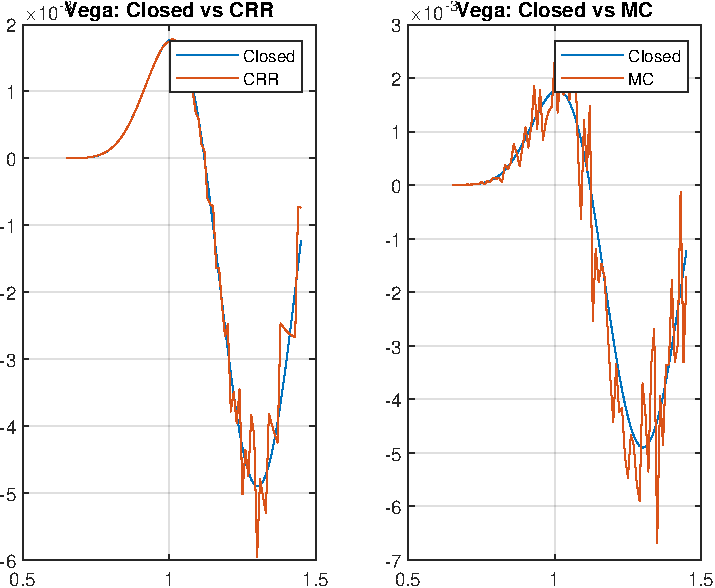
\includegraphics[width=0.7\linewidth]{imgs/vega.pdf}
    \caption{In blue: Vega of the Barrier, computing with the closed formula. Left: Vega approximated with tree based approach. Right: Vega approximated with Monte Carlo.}
    \label{fig:vega}
\end{figure}

\vspace{1 cm}
\section{Question (f) Antithetic Variables Technique}
Observing the equivalence in law between this two formulas
\begin{equation*}
 F_0 \exp\left(-\frac{\sigma^2}{2} T + \sigma \sqrt{T} \cdot \mathcal{N}(0,1) \right) \sim
F_0 \exp\left(-\frac{\sigma^2}{2} T - \sigma \sqrt{T} \cdot \mathcal{N}(0,1) \right)
\end{equation*}
we generated a sample of $M$ normal random variables, computing the prices corresponding to both the two expressions above. Then we took the averages and used them as Monte Carlo prices.
This technique, called antithetic variables, reduces the variance of the generated prices and is part of broad class of methods known as \textit{variance reduction techniques}, see \cite{Hull}. As consequences, the estimated standard deviation \textit{stdEstim} still scales like $\frac{\bar{\omega}}{\sqrt{M}}$, but the coefficient $\bar{\omega}$ is lower. Plotted on a logarithmic scale, like the one below, this translates to a downward shift and a consequent decreases in the number of iterations required for convergence.

\begin{figure}[H]
    \centering
    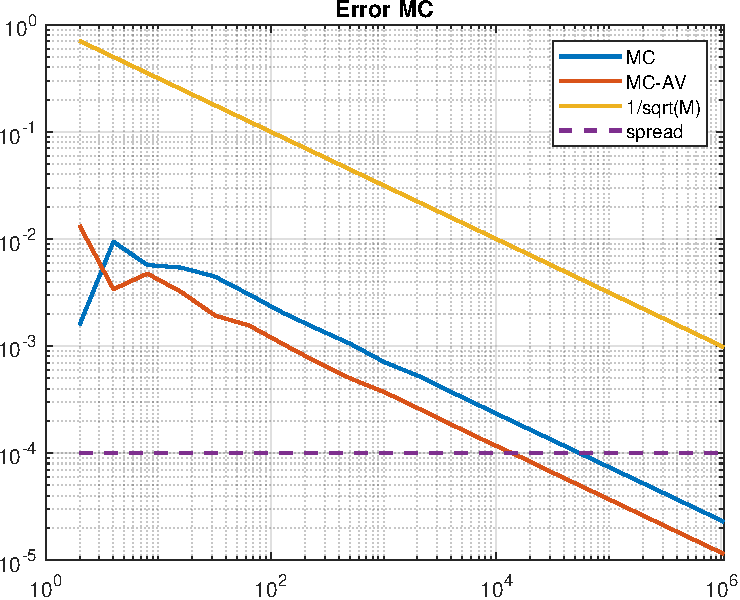
\includegraphics[width=0.7\linewidth]{imgs/antithetic_vars.pdf}
    \caption{Blue line: standard Monte Carlo, same behavior of Figure 1. Orange line: antithetic variable Monte Carlo, reduced variance. The purple line is still the spread, set at $1bp$.}
    \label{fig:antithetic-var}
\end{figure}

\section{Question (g) Bermudan Option Pricing}
We moved on considering a Bermudan Option, where the holder has also the right to exercise it at the end of every month. In order to compute its price we used a CRR approach and at the end of every month we compared the exercise value of each node (payoff of that node) with the continuation value (discounted payoffs of the following time step).

\begin{table}[htpb]
    \centering
    \begin{tabular}{|| c | c ||}
    \hline
        \textbf{Bermudan price} & \textbf{Call price}
        \\0.02880485 & 0.02880214 \\
        28804.85 & 28802.14 \\
    \hline
    \end{tabular}
    \caption{CRR prices of the two options}
    \label{tab:price_b}
\end{table}

As we can see, the two prices do not differ significantly, since early exercise is almost never the optimal choice.

\vspace{1 cm}
\section{Question (h) Bermudan Option Dividend Yield}
By the definition of a Bermudan option, we know that its price lies between the price of a European call and the price of an American call. 
\begin{equation*}
price_{EU} \leq price_{BER} \leq price_{AM}
\end{equation*}

According to the theory, for a Call option that does not pay dividends, the price of a European Call is equal to that of an American Call. Consequently, in the case where $d=0$, we expect the price of the Bermudan option to coincide with that of the European Call.
Varying the dividend yield between 0\% and 5\%, we observe that the two prices tend to be more and more different.

\begin{figure}[htpb]
    \centering
    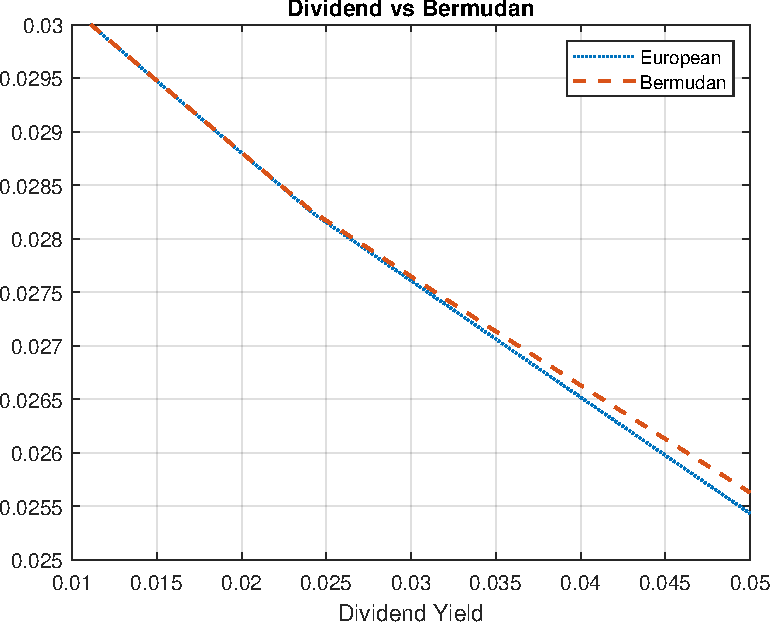
\includegraphics[width=0.8\linewidth]{imgs/dividend_bermudan.pdf}
    \caption{Blue dotted line: European call option. Orange line: Bermudan option. The two are very close for low values of the divided yield; the difference broaden as the dividend grows bigger.}
    \label{fig:bermudan}
\end{figure}


\begin{thebibliography}{9}
\bibitem{hull}
John C. Hull,
\textit{Options, Futures, and Other Derivatives},
Prentice Hall, 7th edition, 2009

\bibitem{crr}
J. Cox, S. Ross and M. Rubenstein,
\textit{Option pricing: A simplified approach}
Journal of Financial Economics, 1979

\bibitem{black}
Fisher Black,
\textit{The pricing of commodity contracts},
Journal of Financial Economics, 1976

\end{thebibliography}